\documentclass{standalone}

\usepackage{tikz}
\usepackage{circuitikz}

\tikzset{block/.style = {draw, fill=white, very thick, rectangle, minimum height=1cm, minimum width=2cm},
         lblock/.style={draw,fill=white,very thick, rectangle, minimum height=3cm, minimum width=1cm},
         sum/.style= {draw, fill=white, very thick, circle, node distance=0.5cm}}

         
\begin{document}
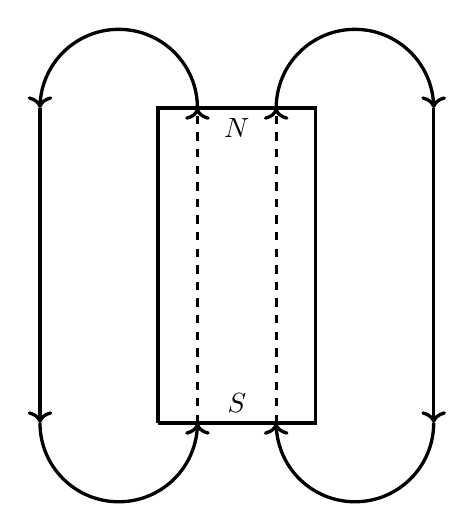
\begin{tikzpicture}[scale=2]
    \draw[-,very thick](0,0)--(0.5,0)node[above]{$S$}--(1,0)--(1,2)--(0.5,2)node[below]{$N$}--(0,2)--(0,0);

    \draw[->,very thick](0.75,2)arc(180:0:0.5);
    \draw[->,very thick](0.25,2)arc(0:180:0.5);
    \draw[->,very thick](1.75,0)arc(0:-180:0.5);
    \draw[->,very thick](-0.75,0)arc(-180:0:0.5);
    

    \draw[->,dashed,very thick](0.25,0)--(0.25,1)--(0.25,2);
    \draw[->,dashed,very thick](0.75,0)--(0.75,1)--(0.75,2);

    \draw[->, very thick](1.75,2)--(1.75,1)--(1.75,0);
    \draw[->, very thick](-0.75,2)--(-0.75,1)--(-0.75,0);
    
\end{tikzpicture}
\end{document}